\subsection{System Identification using P. Hudzovic's method}

An extensive report on the details of P. Hudzovic's method and the accompanied
MATLAB simulations can be found here\cite{ref:comet}.

The method proposed by P. Hudzovic\cite{ref:hudzovic} is based on a model that
approximates a plant with a series of  PT1  elements  multiplied together with
varying time constants $T_k$ to form a PTn element, $G_n(s)$.

\begin{equation}
    G_n(s,r) = K_s\prod_{k=1}^{n}\frac{1}{1+s\cdot T_k(r)}
    \label{eq:pt1_series}
\end{equation}

The neat trick P. Hudzovic proposed was rather than having to find individual,
independent time constants for each PT1 element -- the effort of which greatly
increases with higher orders of $n$  --  one  should  instead  have a function
$T_k(r)$  which  spaces the time constants in a meaningful  way.  He  defines:

\begin{equation}
    T_k(r) = \frac{T}{1-(k-1)r}
    \label{eq:hudzovic}
\end{equation}

where  the  parameter  $r$  must  be confined to  the  interval  $0  \le  r  <
\frac{1}{n-1}$.

With  this  approach  the  problem  has  effectively been reduced  to  finding
appropriate values for $n$,  $T$,  and  $r$  such  that  the  step response of
$G_n(s,r)$  approximates the measured step response as  closely  as  possible.

It is not possible to \textit{directly} calculate these values, however, it is
possible construct a lookup-table from the  equations  \ref{eq:pt1_series} and
\ref{eq:hudzovic} by calculating  a  (theoretically)  infinite  number of step
responses  for  all  values  of  $n$,  $T$,  and $r$, characterising each step
response (i.e. determine $T_u$ and $T_g$),  and performing a reverse lookup on
those  results  to  find  the  parameters  $n$  and  $r$.   This   method   of
reverse-lookup   works   because   the   lookup   curves   are   monotonically
increasing/decreasing (see figure \ref{fig:hudzovic}).


In practice, it is sufficient to calculate about 50 step  response  curves for
each order  $n$  and  interpolate  between  those  points  when performing the
lookup.

Using MATLAB, the lookup table is constructed and the parameters $n$, $r$, and
$T$ are calculated based on  the  previously  determined  parameters $T_u$ and
$T_g$. The  transfer  function  $G_2(s)$  is  calculated  and turns out to be:

\begin{equation}
    G_2(s) = \frac{24.68}{1.159 s^2 + 5.365 s + 1}
\end{equation}

Figure  \ref{fig:hudzovic_step}  shows  the  step response of  the  calculated
transfer  function  $G_2(s)$  and  compares it to the measured step  response.
$G_2(s)$ seems to be a much better approximation  than  the  transfer function
$G_1(s)$ obtained in section \ref{sec:ident_Tt_PT1}.


By looking  at  the Bode-Diagram of the transfer function $G_2(s)$ (see figure
\ref{fig:hudzovic_bode}), we see one potential issue: This system  is a second
order system, which means  the  phase never exceeds \SI{180}{\degree} and thus
the parameter $K_{p,crit}$ cannot be  determined  for  any finite value of the
P-controller's gain! As a result, it will not be possible to use the method of
Ziegler-Nichols for determining controller parameters.

\begin{figure}
    \centering
    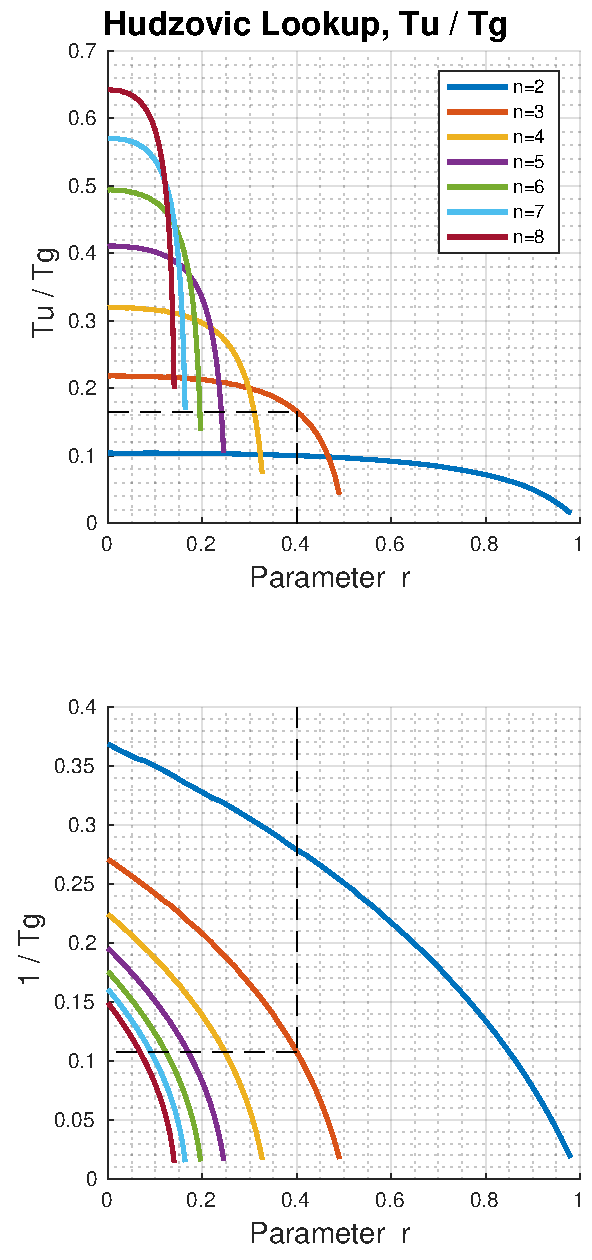
\includegraphics[width=\imagewidth]{images/hudzovic_curves_tu_tg.pdf}
    \caption{Lookup curves generated with P. Hudzovic's equations. By measuring $T_u$ and $T_g$ it is possible to look up the parameters $n$, $r$ and $T$ which can be used together with equation \ref{eq:pt1_series} to construct an accurate transfer function of the measured system.}
    \label{fig:hudzovic}
\end{figure}

\begin{figure}
    \centering
    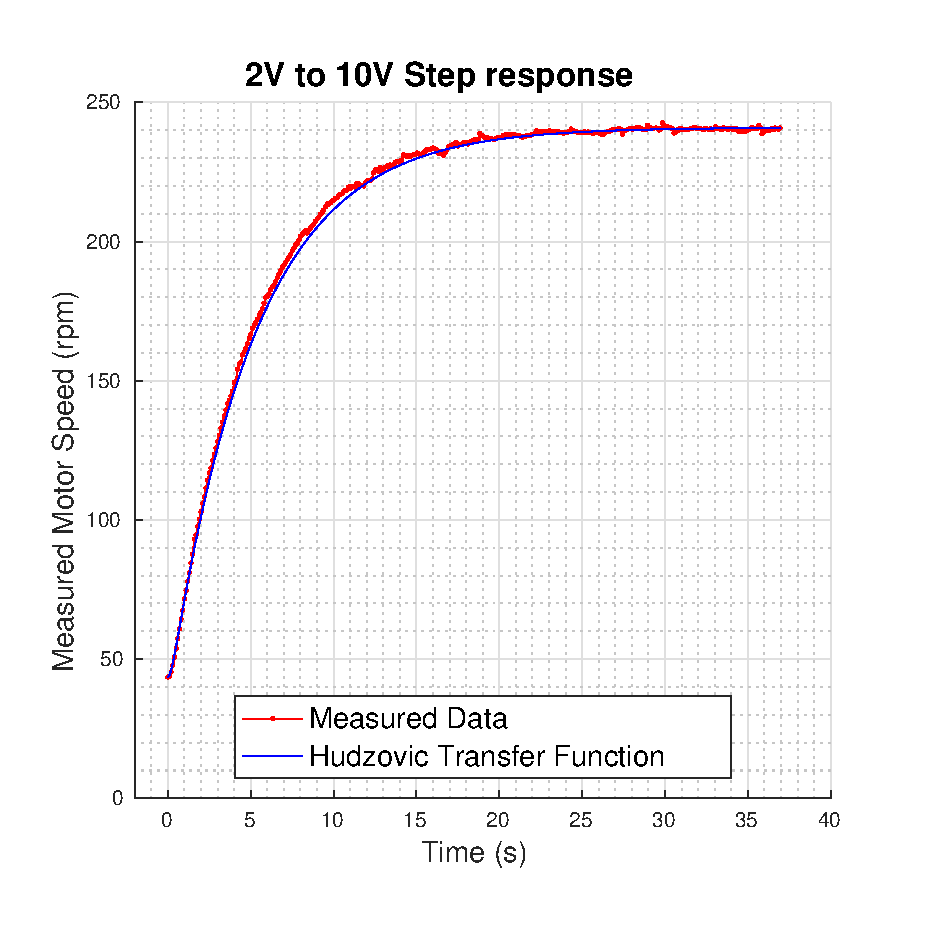
\includegraphics[width=\linewidth]{images/hudzovic}
    \caption{Comparison of the calculated step response function $G_2(s)$ (using P. Hudzovic's method) and the measured step response of the motor.}
    \label{fig:hudzovic_step}
\end{figure}

\begin{figure}
    \centering
    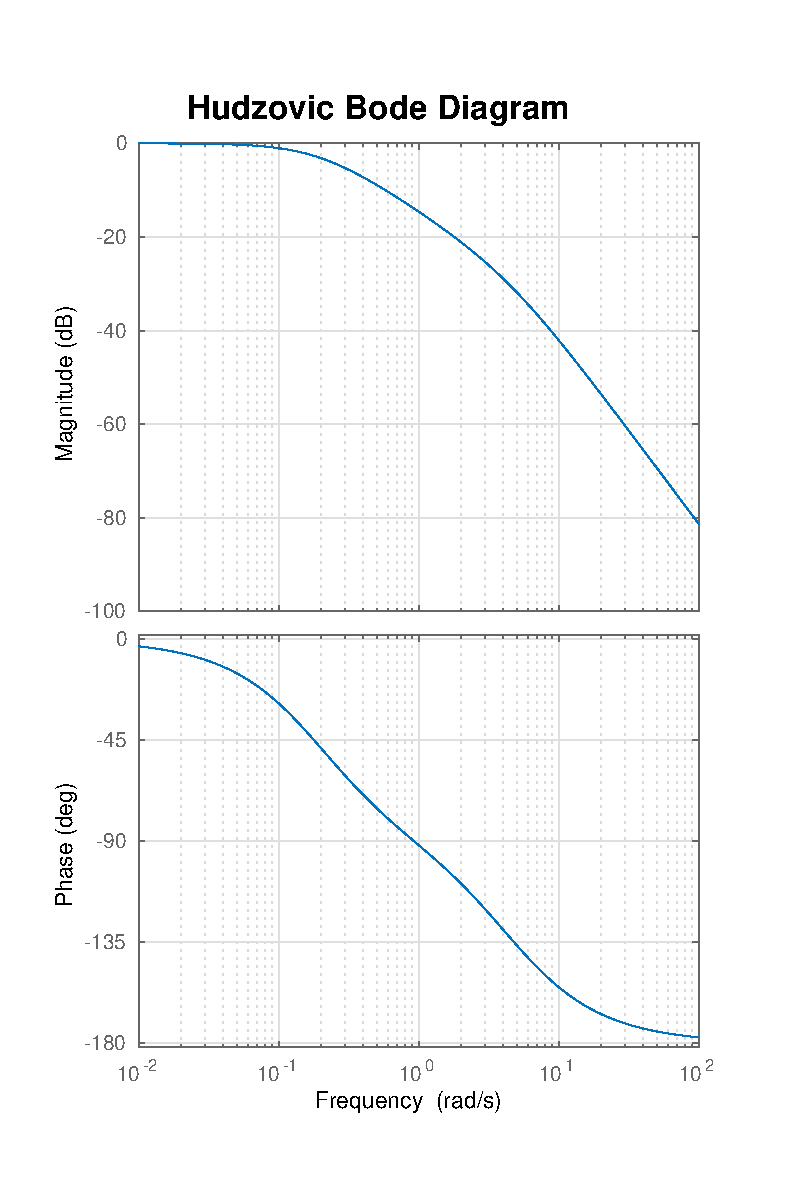
\includegraphics[width=\linewidth]{images/hudzovic_bode}
    \caption{Bode-Diagram of the transfer function $G_2(s)$, acquired using P. Hudzovic's method}
    \label{fig:hudzovic_bode}
\end{figure}

\clearpage
